\documentclass[final_project_1.tex]{subfiles}
\begin{document}
\paragraph{}
With Glivenko-Cantelli theorem, the uniform LLN is guaranteed through the convergence of Kolmogorov statistics. With Donsker theorem, the uniform CLT is guaranteed and thus we know the asymptotic behaviour of Kolmogorov statistics. In the previous discussion, we consider the setting that the underlying distribution is known. However, in real life, this is not the case! What we have is the empirical distribution and some assumption about the random source. And our goal is to find out the underlying distribution. With the help of Donsker theorem, we can construct a confidence interval of Kolmogorov statistics and draw inference about the empirical process. And finally test whether our assumption on the true distribution is correct with high probability.

\subsection{Framework}

\paragraph{}
Kolmogorov-Smirov test is a famous non-parametric goodness of fitting test. The test consider the Kolmogorov statistics: $D_n = \sup_{x\in \mathcal{R}}|\hat{F}_n(x)-F(x)|$, which is a {\it distribution-free} statistics. The convergence of $D_n$ provides us a way to see that whether a source is sampled from the guessing distribution or not. Moreover, since the probability distribution of $D_n$ will converge to that of a Brownian Bridge, the confidence interval can be calculated.


\subsection{Convergence of Kolmogorov Statistics}

\paragraph{}
Donsker theorem says that the Kolmogorov statistics will converge in distribution to the spremum of a Brownian bridge. To prove this, we prove a stronger result:
\begin{theorem}
Let $E_n$ be an empirical process with $n$ samples and $\mathbf{B}=\{B_t:t\in[0,1]\}$ be a Brownian bridge. Then for all $t\in[0,1]$, $E_n(t)\rightarrow B_t$ almost surely as $n\rightarrow\infty$.
\end{theorem}

To prove this theorem, we need three steps:
\begin{enumerate}
\item $E_n$ converge to $\mathbf{B}$ almost surely on {\bf finite} many of points in [0,1] as $n\rightarrow \infty$.
\item $E_n$ with {\bf finite} many of points in [0,1] will define the original empirical process as the number of points grows to infinity.
\item $\mathbf{B}$ with {\bf finite} many of points in [0,1] will define the original Brownian bridge as the number of points grows to infinity.
\end{enumerate}

For 2 and 3, Daniell-Kolmogorov extension theorem guaranteed the convergence. Since this is out of the discussion of this project, so we will not prove it here. However, if you are interested with it, you can find lots of resource on the internet.

As a result, our goal here is to show that the empirical process $E_n$ will converge to the Brownian bridge $\mathbf{B}$ almost surely on {\bf finite} many of points in [0,1] as $n\rightarrow \infty$.

\begin{proof}
First, recall the {\it Probability integral transform theorem} that the distribution of the  CDF(cumulative distribution function) transform of any random variable is uniform on [0,1]. As a result, we can consider the empirical process of uniform distribution case first. As to the empirical process of general distribution function $F$, we can simply compose the $F(x)$ term to the result of uniform case. Details will be explained later.

So let's consider $n$ uniform $i.i.d.$ random variables $X_1, X_2, ..., X_n$ from $F(x)=x$ on [0,1] and use them to construct an empirical distribution $\hat{F}_n$. Now take arbitrary $k$ points $x_1, x_2, ..., x_k$ in [0,1]. We observe the behaviour on these $k$ finite points. Represent them in a random vector:

\[ \sqrt{n} \left[ \begin{array}{c}
\hat{F}_n(x_1)-F(x_1) \\
\vdots \\
\hat{F}_n(x_k)-F(x_k) \end{array} \right]=
\frac{1}{\sqrt{n}}\sum^n_{i=1}
\left[ \begin{array}{c}
{\bf I}\{X_i\leq x_1\} - F(x_1) \\
\vdots \\
{\bf I}\{X_i\leq x_k\} - F(x_k)
\end{array} \right]:=
\frac{1}{\sqrt{n}}
\sum^n_{i=1}{\bf Z}_i
\]

where ${\bf Z}_1, {\bf Z}_2, ..., {\bf Z}_n$ are $i.i.d.$ $k$-dimensional random vectors with $E[{\bf Z}_i]={\bf 0}$ and $Cov[{\bf Z_i}]={\bf Q}\ \forall i$, and {\bf Q} is the covariance matrix such that
$${\bf Q}_{i,i} = F(x_i)[1-F(x_i)]$$
and
$${\bf Q}_{i,j}=F(x_i\wedge x_j)-F(x_i)F(x_j)=x_i\wedge x_j - x_ix_j$$

Note that the random part is in the random variables $X_1, ..., X_n$, that is, the empirical distribution $\hat{F}_n$. Not the arbitrary points $x_1, x_2, ..., x_k$.

Then, by the multinomial central limit theorem, $\frac{1}{\sqrt{n}}\sum^n_{i=1}{\bf Z}_i$ converges in distribution to $N_k({\bf 0}, {\bf Q})$. In other words, 
\[\left[ \begin{array}{c}
E_n(x_1)\\
\vdots\\
E_n(x_k)
\end{array} \right]
\xrightarrow{d}\left[ \begin{array}{c}
W(x_1)\\
\vdots\\
W(x_k)
\end{array}\right]
\]
where {\bf W} = ($W_1, W_2, ..., W_k$)'$\sim N_k({\bf 0}, {\bf Q})$.

Also, by the {\it Uniqueness Property} of Gaussian process and the property of {\bf Q}, we can know that $W(x_i)=B(x_i)\ \forall i$, where $B$ is a Brownian bridge. That is, the empirical process will converge to a Brownian bridge at finite points $x_1, x_2, ..., x_k$. Thus, 1 has been proved!

To sum up, the empirical process of uniform distribution will converge to the Brownian bridge in finite many points. Also, by Daniell-Kolmogorov extension theorem, finite many points of distributions will define a stochastic process. And for ($E_n(x_1), E_n(x_2), ..., E_n(x_k)$) and ($B(x_1)m B(x_2), ..., B(x_k)$) will define the empirical process of uniform distribution and Brownian bridge respectively. The following 
\begin{figure}[ht]
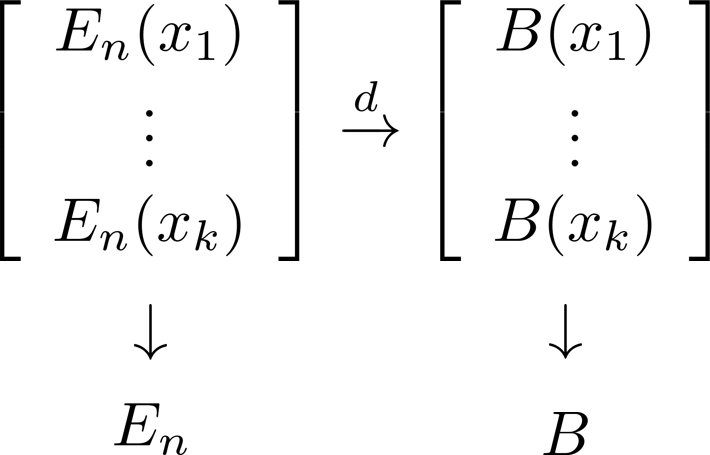
\includegraphics[scale=0.4]{donsker_1.png}
\caption{Proof flow of Theorem 6}
\end{figure}
\end{proof}

Finally, let's put everything together. First, since $E_n\rightarrow B$, it's clearly that
$$\sup_{0\leq x\leq 1}|E_n(x)|\xrightarrow{d}\sup_{0\leq x\leq 1}|B(x)|$$

Namely, the Kolmogorov statistics of the uniform distribution on [0,1] will converge in distribution to the absolute supremum norm of a Brownian bridge.

As to general distribution $F$. Let $G$ denotes the uniform distribution on [0, 1]. Consider the Kolmogorov statistics
\begin{align*}
D_n:&=\sqrt{n}\sup_{0\leq x\leq 1}|\hat{F}_n(x) - F(x)|\\
&=\sqrt{n}\sup_{0\leq x\leq 1}|G[\hat{F}_n(x)] - G[F(x)]|\\
&\xrightarrow{d}\sup_{0\leq x\leq 1}|B(F(x))|
\end{align*}

This is the Donsker Theorem, the uniform central limit theorem for empirical process.

\end{document}